% !TeX TXS-program:compile = txs:///pdflatex/[--shell-escape]

\documentclass[11pt, letterpaper]{article}

\usepackage[utf8]{inputenc}
\usepackage{minted}
\usepackage[T1]{fontenc}
\usepackage{lmodern}
\usepackage{graphicx}
\usepackage{longtable}
\usepackage{wrapfig}
\usepackage{rotating}
\usepackage{amsmath}
\usepackage{textcomp}
\usepackage{amssymb}
\usepackage{hyperref}
\usepackage[spanish]{babel}
\usepackage[round]{natbib}
\usepackage{subcaption}

\title{\bfseries Tarea}
\author{Ángel García Báez}
\date{\today}
\setcounter{tocdepth}{4} 

\begin{document}
	
	% Página de presentación
	\begin{titlepage}
		\centering
		
\includegraphics[width=0.2\textwidth]{logo.png}\par
		\vspace{1cm}
		{\LARGE \bfseries Universidad Veracruzana \par}
		\vspace{1cm}
		{\Large Maestría en Inteligencia Artificial\par}
		\vspace{3cm}
		{\LARGE \bfseries Lógica difusa \par}
		\vspace{1cm}
		{\Large \bfseries Tarea 2. Problema del mesero y problema del confort con lógica difusa programado paso a paso en MATLAB. \par}
		\vfill
		{\Large \textit{Ángel García Báez}\par}
		\vfill
		{\Large Dr. Sergio Hernández Méndez \par}
		\vfill
		{\Large \today \par}
	\end{titlepage}
	
	% Página exclusiva para la tabla de contenidos
	\newpage
	\tableofcontents
	\newpage
	
% Explicación breve

\section{Introducción}

En el presente reporte se anexan los resultados del problema del mesero y el problema del confort planteados en clase con salidas singleton, modelados y evaluados con el fuzzy toolbox de matlab así como el contraste con una implementación del código hecha paso por paso para contrastar los resultados en 3 escenarios distintos por cada problema: Cuando las 2 condiciones son mínimas, cuando son medias y cuando son máximas.

\newpage


\section{Problema 1: Problema del mesero}

\subsection{Explicación del Problema}

Se tiene el problema de determinar cuanta propina dejarle a un mesero en un restaurante después de comer. Para ello, se toman en cuenta las variables de Servicio y la Comida.

En la tarea 1, se hizo la labor de probar con distintas combinaciones de funciones de membresía y parámetros para suavizar lo más posible la curva, a continuación se muestra el mejor caso con salidas singleton al que se llego después de dichas experimentaciones:

\subsection{Variables y sus codificaciones}

A continuación se listan los valores de las variables lingüísticas que se
propusieron para SERVICIO, COMIDA y PROPINA como sigue:

\begin{enumerate}
	\item Servicio: Malo ($\mu = 1.5$, $\sigma = 2$), Regular ($\mu = 5$, $\sigma = 1.5$) y Bueno ($\mu = 7.5$, $\sigma = 1.5$).
	\begin{figure}[h]
		\centering
		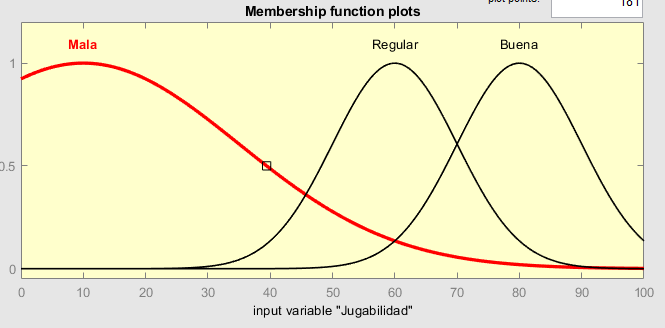
\includegraphics[width=0.8\textwidth]{IMG/P11.png}
	\end{figure}
	
	\newpage
	
	\item Comida: Malo ($\mu = 15$, $\sigma = 15$), Normal ($\mu = 45.5$, $\sigma = 15$), Buena ($\mu = 66$, $\sigma = 10$) y Excelente ($\mu = 90$, $\sigma = 15$).
	\begin{figure}[h]
		\centering
		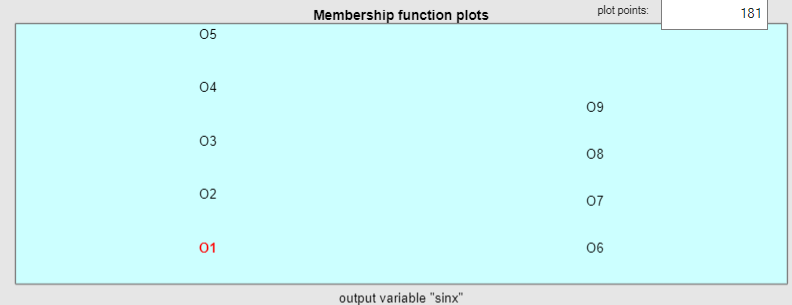
\includegraphics[width=0.8\textwidth]{IMG/P12.png}
	\end{figure}
	
	\item Baja (valor de 5), Normal (valor de 12) y Alta (valor de 16).
	\begin{figure}[h]
		\centering
		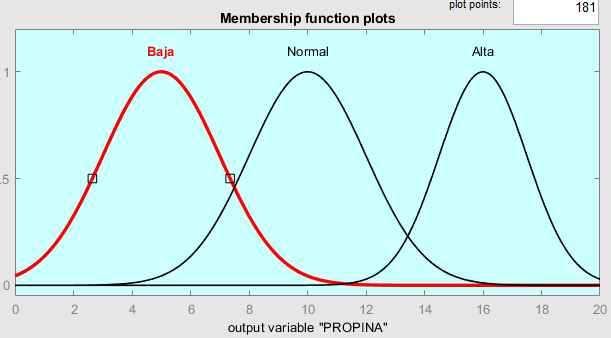
\includegraphics[width=0.8\textwidth]{IMG/P13.png}
	\end{figure}
\end{enumerate}

Las funciones de membresía de SERVICIO y COMIDA fueron modeladas con Gaussianas, mientras que la salida de PROPINA fue modelada con singletons (una triangular modificada en 1 solo valor) para mantener el sistema $sencillo$ y por su naturaleza discreta. \\

Se mantuvo el método de desfuzzificación del centroide (centro de masa) para todas las funciones con la inferencia de Mandani.\\

\newpage

\subsection{Reglas de inferencia.}

A continuación se muestran las doce reglas que se construyeron para este problema:

\begin{enumerate}
	\item R1: Si \textbf{SERVICIO} es \textbf{\textit{MALO}} y la \textbf{COMIDA} es \textbf{\textit{MALA}}, la \textbf{PROPINA} es \textbf{\textit{BAJA}}.
	\item R2: Si \textbf{SERVICIO} es \textbf{\textit{BUENO}} y la \textbf{COMIDA} es \textbf{\textit{NORMAL}}, la \textbf{PROPINA} es \textbf{\textit{NORMAL}}.
	\item R3: Si \textbf{SERVICIO} es \textbf{\textit{REGULAR}} y la \textbf{COMIDA} es \textbf{\textit{NORMAL}}, la \textbf{PROPINA} es \textbf{\textit{NORMAL}}.
	\item R4: Si \textbf{SERVICIO} es \textbf{\textit{REGULAR}} y la \textbf{COMIDA} es \textbf{\textit{BUENA}}, la \textbf{PROPINA} es \textbf{\textit{NORMAL}}.
	\item R5: Si \textbf{SERVICIO} es \textbf{\textit{BUENO}} y la \textbf{COMIDA} es \textbf{\textit{EXCELENTE}}, la \textbf{PROPINA} es \textbf{\textit{ALTA}}.
	\item R6: Si \textbf{SERVICIO} es \textbf{\textit{MALO}} y la \textbf{COMIDA} es \textbf{\textit{EXCELENTE}}, la \textbf{PROPINA} es \textbf{\textit{BAJA}}.
	\item R7: Si \textbf{SERVICIO} es \textbf{\textit{BUENO}} y la \textbf{COMIDA} es \textbf{\textit{MALA}}, la \textbf{PROPINA} es \textbf{\textit{BAJA}}.
	\item R8: Si \textbf{SERVICIO} es \textbf{\textit{MALO}} y la \textbf{COMIDA} es \textbf{\textit{NORMAL}}, la \textbf{PROPINA} es \textbf{\textit{BAJA}}.
	\item R9: Si \textbf{SERVICIO} es \textbf{\textit{MALO}} y la \textbf{COMIDA} es \textbf{\textit{BUENA}}, la \textbf{PROPINA} es \textbf{\textit{BAJA}}.
	\item R10: Si \textbf{SERVICIO} es \textbf{\textit{BUENO}} y la \textbf{COMIDA} es \textbf{\textit{BUENA}}, la \textbf{PROPINA} es \textbf{\textit{ALTA}}.
	\item R11: Si \textbf{SERVICIO} es \textbf{\textit{REGULAR}} y la \textbf{COMIDA} es \textbf{\textit{MALA}}, la \textbf{PROPINA} es \textbf{\textit{BAJA}}.
	\item R12: Si \textbf{SERVICIO} es \textbf{\textit{REGULAR}} y la \textbf{COMIDA} es \textbf{\textit{EXCELENTE}}, la \textbf{PROPINA} es \textbf{\textit{ALTA}}.
\end{enumerate}

\newpage

\subsection{Gráficos del problema 1}

La gráfica de superficie resultante de todo lo descrito previamente, es la siguiente:

\begin{figure}[h]
	\centering
	\begin{subfigure}{0.42\textwidth} % Reducido de 0.45
		\centering
		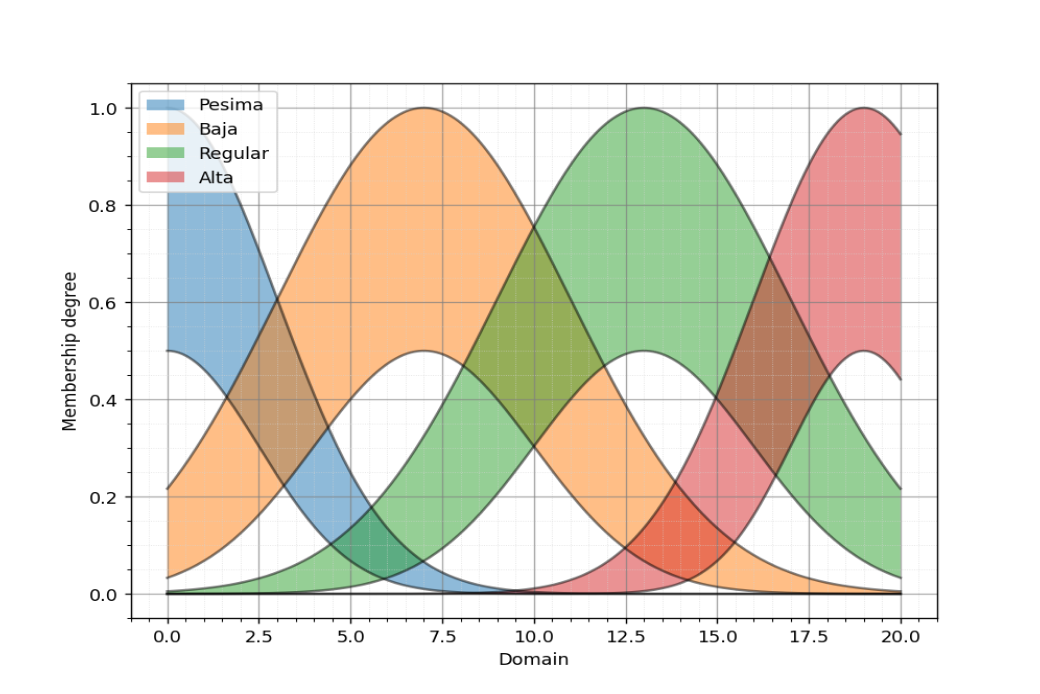
\includegraphics[width=1.3\textwidth]{IMG/P14.png}
		\label{fig:G1}
	\end{subfigure}
	\hfill
	\begin{subfigure}{0.42\textwidth} % Reducido de 0.45
		\centering
		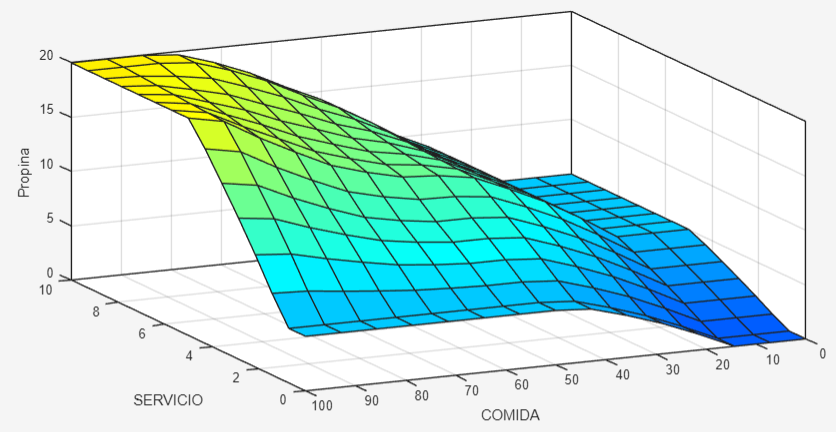
\includegraphics[width=1.2\textwidth]{IMG/P15.png}
		\label{fig:G2}
	\end{subfigure}
	\label{fig:comparacion1}
\end{figure}

Se observa como la gráfica producida por la combinación de distribuciones Gaussianas y la salidas singleton resulta tener un comportamiento suave en el descenso de sus valores.

\newpage

\subsection{Implementación del problema 1 paso a paso}

Como se menciono en un inicio, el principal objetivo de esta actividad es implementar uno mismo el sistema de lógica difusa para comparar los resultados con respecto de los mostrados por el fuzzy toolbox de matula.\\

El primer paso  identificar las variables de discurso SERVICIO, COMIDA y PROPINA para inicializarlas en 0.\\

Con referencia a lo explicado en el libro de \cite{Cisneros2004}, se implemento la función de membresía Gaussiana tal y como la define a continuación:

\[
f(x, \mu, \sigma) = e^{\left( \frac{(x - \mu)^2}{2\sigma^2} \right)}
\]

Posteriormente, se definieron los rangos de cada una de las funciones de membresía, dado que solo se usan funciones gaussianas y singletons, se dejaron los rangos tal cual se había presentado anteriormente:

\begin{enumerate}
	\item Servicio: Malo ($\mu = 1.5$, $\sigma = 2$), Regular ($\mu = 5$, $\sigma = 1.5$) y Bueno ($\mu = 7.5$, $\sigma = 1.5$).
	\item Comida: Malo ($\mu = 15$, $\sigma = 15$), Normal ($\mu = 45.5$, $\sigma = 15$), Buena ($\mu = 66$, $\sigma = 10$) y Excelente ($\mu = 90$, $\sigma = 15$).	
	\item Baja (valor de 5), Normal (valor de 12) y Alta (valor de 16).
\end{enumerate} 



Siguiendo con el proceso, fueron implementadas cada una las 12 reglas que ya se mostraron previamente, haciendo uso de la operación de conjuntos difusos $AND$, para esto, la activación de las reglas del sistema se determinan de la siguiente forma:

\[
\text{Activación de regla}  = \min( \mu_A(X), \mu_B(Y) )
\]

\newpage

Por ultimo, ya que se contaban con las funciones de membresía y el sistema de reglas, dado que se van a trabajar con salidas singleton, la forma de deffuzificar las entradas para generar las salidas es mediante el método del centro de masa que se describe en el libro como sigue:


$$
\text{Crisp} = \frac{\sum_{i=1}^{n} x_i \cdot \mu(x_i)}{\sum_{i=1}^{n} \mu(x_i)}
$$

donde:

\begin{itemize}
	\item \( x_i \) son los valores discretos de la variable de salida.
	\item \( \mu(x_i) \) es el grado de pertenencia de \( x_i \) en la función de pertenencia de la salida difusa.
	\item \( n \) es el número total de puntos discretos en el dominio de salida.
\end{itemize}

Una vez que el sistema esta listo y programado, se procede a hacer la comparativa con el toolbox de matlab.

\newpage

\subsection{Comparativa para el problema 1}

A continuación se presentan los resultados que da el sistema programado paso a paso en matlab contra el resultado para el mismo sistema por parte del fuzzy toolbox en 3 escenarios distintos.

\subsubsection{Caso mínimo}

Para el caso mínimo, se propone un $SERVICIO = 0$ y una $COMIDA = 0$ para ver como se comportan ambas versiones ante situaciones tan extremas.

\begin{figure}[h]
	\centering
	\begin{subfigure}{0.40\textwidth} % Reducido de 0.45
		\centering
		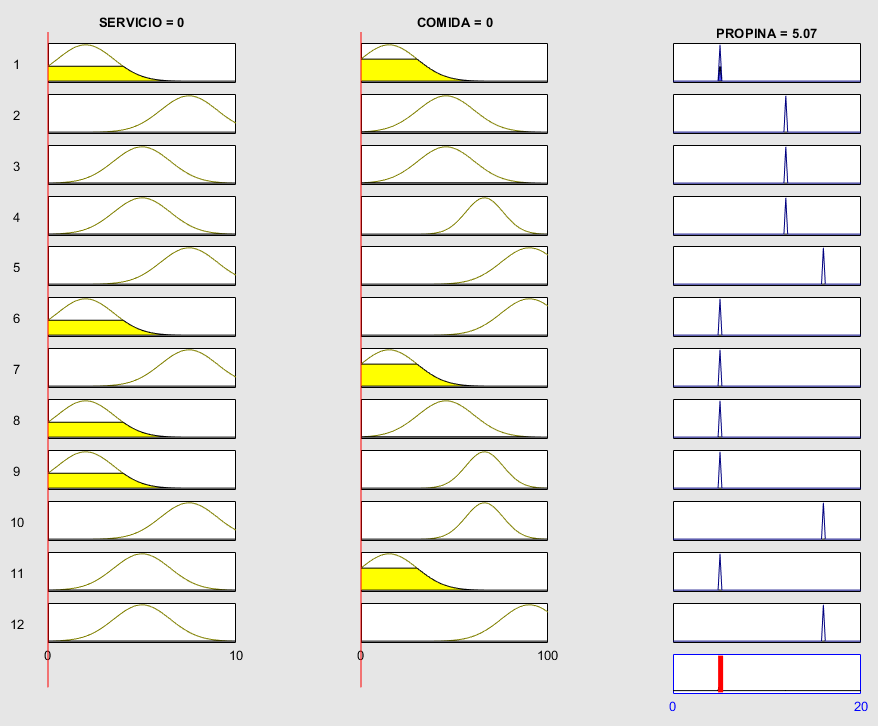
\includegraphics[width=1.4\textwidth]{IMG/RP11.png}
		\label{fig:G3}
	\end{subfigure}
	\hfill
	\begin{subfigure}{0.42\textwidth} % Reducido de 0.45
		\centering
		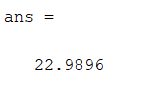
\includegraphics[width=0.8\textwidth]{IMG/M11.png}
		\label{fig:G4}
	\end{subfigure}
	\label{fig:comparacion2}
\end{figure}

A la izquierda se muestran los resultados del toolbox y a la derecha el resultado del sistema programado paso a paso. El toolbox reporta un valor de 5.07 para el caso planteado, mientras que el sistema programado paso a paso muestra un valor de 5.0003. La diferencia entre ambos casos es mínima (menos de una unidad), por lo que se puede afirmar que llegan al mismo resultado. Un servicio de 0 y una comida de 0 llegan a dar como resultado una propina de 5.035\% en promedio (baja).

\newpage

\subsubsection{Caso medio}
Para el caso mínimo, se propone un $SERVICIO = 4$ y una $COMIDA = 52$ para ver como se comportan ambas versiones ante situación media.

\begin{figure}[h]
	\centering
	\begin{subfigure}{0.40\textwidth} % Reducido de 0.45
		\centering
		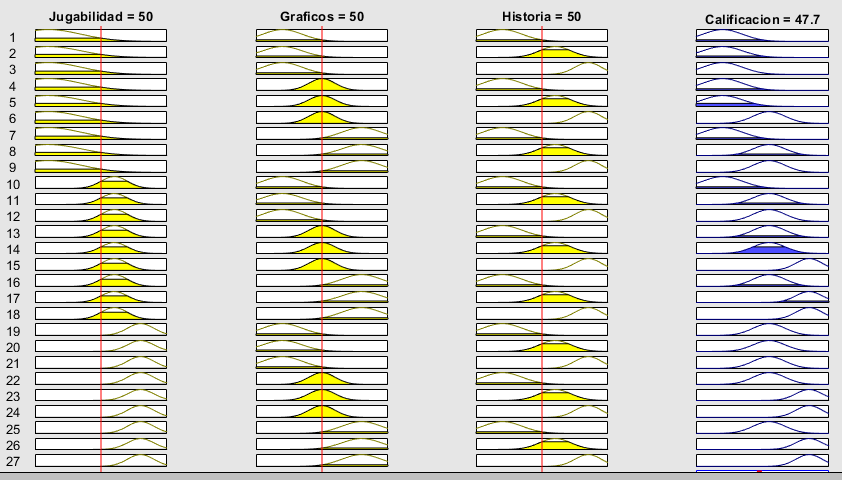
\includegraphics[width=1.4\textwidth]{IMG/RP12.png}
		\label{fig:G5}
	\end{subfigure}
	\hfill
	\begin{subfigure}{0.42\textwidth} % Reducido de 0.45
		\centering
		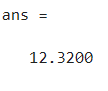
\includegraphics[width=0.8\textwidth]{IMG/M12.png}
		\label{fig:G6}
	\end{subfigure}
	\label{fig:comparacion3}
\end{figure}

A la izquierda se muestran los resultados del toolbox y a la derecha el resultado del sistema programado paso a paso. El toolbox reporta un valor de 9.95 para el caso planteado, mientras que el sistema programado paso a paso muestra un valor de 9.8469. La diferencia entre ambos casos es mínima (menos de una unidad), por lo que se puede afirmar que llegan al mismo resultado. Un servicio de 4 y una comida de 52 llegan a dar como resultado una propina de 9.9\% en promedio (media).

\newpage

\subsubsection{Caso máximo}
Para el caso mínimo, se propone un $SERVICIO = 10$ y una $COMIDA = 100$ para ver como se comportan ambas versiones ante situaciones tan extremas.

\begin{figure}[h]
	\centering
	\begin{subfigure}{0.40\textwidth} % Reducido de 0.45
		\centering
		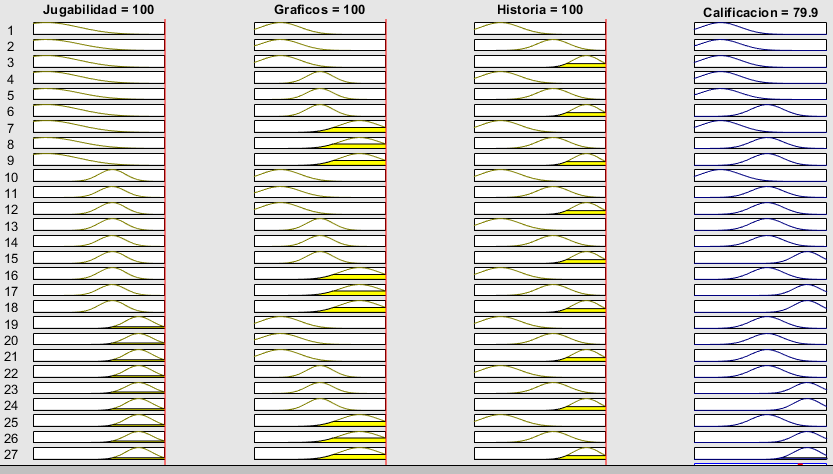
\includegraphics[width=1.4\textwidth]{IMG/RP13.png}
		\label{fig:G7}
	\end{subfigure}
	\hfill
	\begin{subfigure}{0.42\textwidth} % Reducido de 0.45
		\centering
		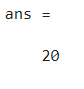
\includegraphics[width=0.8\textwidth]{IMG/M13.png}
		\label{fig:G8}
	\end{subfigure}
	\label{fig:comparacion4}
\end{figure}

A la izquierda se muestran los resultados del toolbox y a la derecha el resultado del sistema programado paso a paso. El toolbox reporta un valor de 16 para el caso planteado, mientras que el sistema programado paso a paso muestra un valor de 15.9992. La diferencia entre ambos casos es mínima, por lo que se puede afirmar que llegan al mismo resultado. Un servicio de 10 y una comida de 100 llegan a dar como resultado una propina del 16 \% (Alta) haciendo el redondeo.

\newpage

\section{Problema 2: Problema del confort}

\subsection{Explicación del Problema}

Se tiene el problema más especifico de determinar el confort que tiene una persona dadas las variables  de temperatura y humedad en el ambiente.

En la tarea 1, se hizo la labor de probar con distintas combinaciones de funciones de membresía y parámetros para suavizar lo más posible la curva, a continuación se muestra el mejor caso con salidas singleton al que se llego después de dichas experimentaciones:

\subsection{Variables y sus codificaciones}

A continuación se listan los valores de las variables lingüísticas que se propusieron para TEMPERATURA, HUMEDAD y COMFORT como sigue:

\begin{enumerate}
	\item Temperatura: Frio ($\mu = 0$, $\sigma = 3$), Fresco ($\mu = 11$, $\sigma = 3$), Idóneo ($\mu = 18$, $\sigma = 2.5$) y Calurosa ($\mu = 26$, $\sigma = 3$).
	\begin{figure}[h]
		\centering
		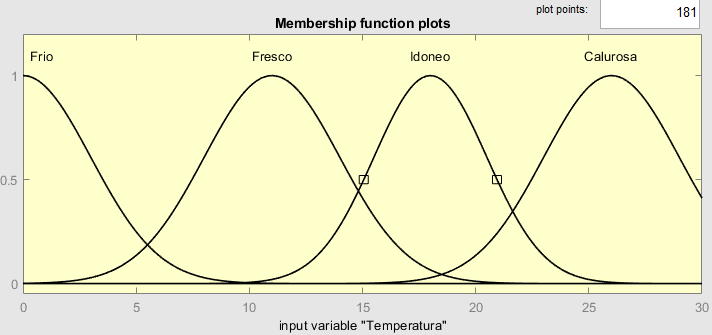
\includegraphics[width=0.8\textwidth]{IMG/P21.png}
	\end{figure}
	\newpage
	\item Humedad: Baja ($\mu = 20$, $\sigma = 10$), Media ($\mu = 40$, $\sigma = 15$) y Alta ($\mu = 80$, $\sigma = 15$).
	\begin{figure}[h]
		\centering
		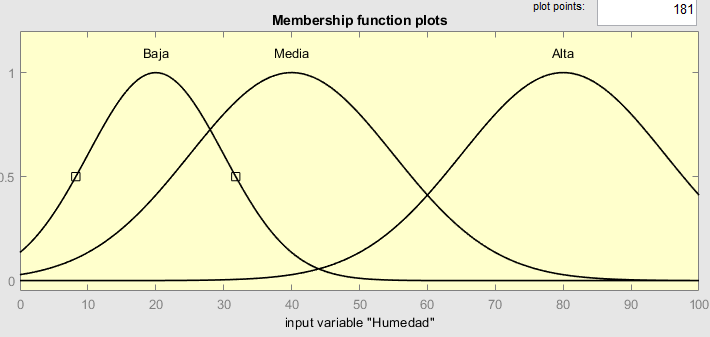
\includegraphics[width=0.8\textwidth]{IMG/P22.png}
	\end{figure}
	\item Confort: Malo (Valor = 2), Incomodo (Valor = 4) y Comoda (Valor = 2).
	\begin{figure}[h]
		\centering
		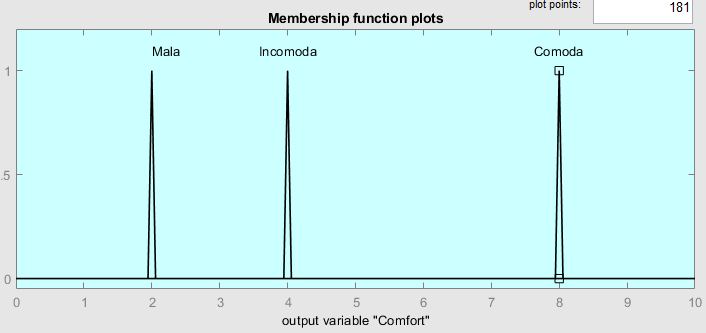
\includegraphics[width=0.8\textwidth]{IMG/P23.png}
	\end{figure}
\end{enumerate}


Las funciones de membresía de TEMPERATURA y HUMEDAD fueron modeladas con Gaussianas, mientras que la salida de CONFORT fue modelada con singletons (una triangular modificada en 1 solo valor) para mantener el sistema $sencillo$ y por su naturaleza discreta. \\

Se mantuvo el método de desfuzzificación del centroide (centro de masa) para todas las funciones con la inferencia de Mandani.\\

\newpage

\subsection{Reglas de inferencia.}

A continuación se muestran las 10 reglas que se construyeron para este problema:

\begin{enumerate}
	\item R1: Si \textbf{TEMPERATURA} es \textbf{\textit{FRÍO}} y la \textbf{HUMEDAD} es \textbf{\textit{BAJA}}, el \textbf{CONFORT} es \textbf{\textit{INCÓMODA}}.
	\item R2: Si \textbf{TEMPERATURA} es \textbf{\textit{FRESCO}} y la \textbf{HUMEDAD} es \textbf{\textit{BAJA}}, el \textbf{CONFORT} es \textbf{\textit{CÓMODA}}.
	\item R3: Si \textbf{TEMPERATURA} es \textbf{\textit{IDÓNEO}} y la \textbf{HUMEDAD} es \textbf{\textit{BAJA}}, el \textbf{CONFORT} es \textbf{\textit{CÓMODA}}.
	\item R4: Si \textbf{TEMPERATURA} es \textbf{\textit{FRÍO}} y la \textbf{HUMEDAD} es \textbf{\textit{MEDIA}}, el \textbf{CONFORT} es \textbf{\textit{CÓMODA}}.
	\item R5: Si \textbf{TEMPERATURA} es \textbf{\textit{IDÓNEO}} y la \textbf{HUMEDAD} es \textbf{\textit{MEDIA}}, el \textbf{CONFORT} es \textbf{\textit{MALA}}.
	\item R6: Si \textbf{TEMPERATURA} es \textbf{\textit{FRÍO}} y la \textbf{HUMEDAD} es \textbf{\textit{BAJA}}, el \textbf{CONFORT} es \textbf{\textit{INCÓMODA}}.
	\item R7: Si \textbf{TEMPERATURA} es \textbf{\textit{IDÓNEO}} y la \textbf{HUMEDAD} es \textbf{\textit{ALTA}}, el \textbf{CONFORT} es \textbf{\textit{INCÓMODA}}.
	\item R8: Si \textbf{TEMPERATURA} es \textbf{\textit{CALUROSA}} y la \textbf{HUMEDAD} es \textbf{\textit{BAJA}}, el \textbf{CONFORT} es \textbf{\textit{MALA}}.
	\item R9: Si \textbf{TEMPERATURA} es \textbf{\textit{CALUROSA}} y la \textbf{HUMEDAD} es \textbf{\textit{MEDIA}}, el \textbf{CONFORT} es \textbf{\textit{INCÓMODA}}.
	\item R10: Si \textbf{TEMPERATURA} es \textbf{\textit{CALUROSA}} y la \textbf{HUMEDAD} es \textbf{\textit{ALTA}}, el \textbf{CONFORT} es \textbf{\textit{MALA}}.
\end{enumerate}


\newpage

\subsection{Gráficos del problema 2}

La gráfica de superficie resultante del sistema que modela el problema del confort térmico es la siguiente:

\begin{figure}[h]
	\centering
	\begin{subfigure}{0.42\textwidth} % Reducido de 0.45
		\centering
		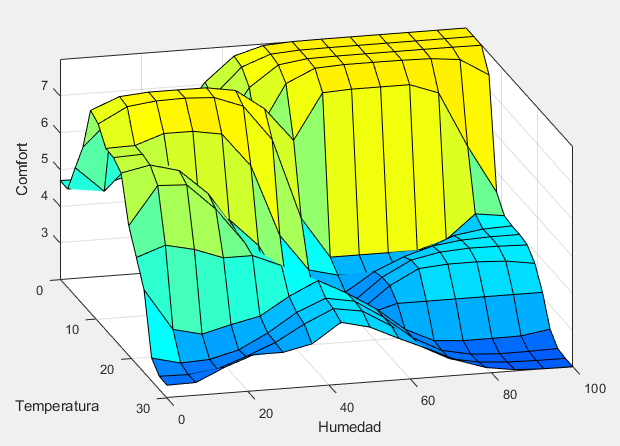
\includegraphics[width=1.3\textwidth]{IMG/P24.png}
		\label{fig:G10}
	\end{subfigure}
	\hfill
	
	\begin{subfigure}{0.42\textwidth} % Reducido de 0.45
		\centering
		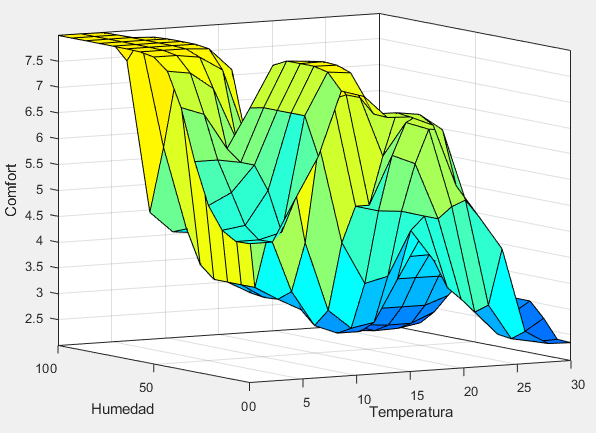
\includegraphics[width=1.2\textwidth]{IMG/P25.png}
		\label{fig:G11}
	\end{subfigure}
	\label{fig:comparacion5}
\end{figure}

Se observa como la gráfica producida por la combinación de distribuciones Gaussianas y la salidas presenta cierto comportamiento suave, en la forma de sus descensos, pero aun así presenta cambios abruptos en algunas regiones que no son deseables. 

\newpage

\subsection{Implementación del problema 2 paso a paso}

Como se menciono en un inicio, el principal objetivo de esta actividad es implementar uno mismo el sistema de lógica difusa para comparar los resultados con respecto de los mostrados por el fuzzy toolbox de matlab.\\

El primer paso  identificar las variables de discurso TEMPERATURA, HUMEDAD y CONFORT para inicializarlas en 0.\\

Con referencia a lo explicado en el libro de \cite{Cisneros2004}, se implemento la función de membresía Gaussiana tal y como la define a continuación:

\[
f(x, \mu, \sigma) = e^{\left( \frac{(x - \mu)^2}{2\sigma^2} \right)}
\]

Posteriormente, se definieron los rangos de cada una de las funciones de membresía, dado que solo se usan funciones gaussianas y singletons, se dejaron los rangos tal cual se había presentado anteriormente:

\begin{enumerate}
	\item Temperatura: Frio ($\mu = 0$, $\sigma = 3$), Fresco ($\mu = 11$, $\sigma = 3$), Idóneo ($\mu = 18$, $\sigma = 2.5$) y Calurosa ($\mu = 26$, $\sigma = 3$).
	\item Humedad: Baja ($\mu = 20$, $\sigma = 10$), Media ($\mu = 40$, $\sigma = 15$) y Alta ($\mu = 80$, $\sigma = 15$).
	\item Confort: Malo (Valor = 2), Incomodo (Valor = 4) y Comoda (Valor = 2).
\end{enumerate}

Siguiendo con el proceso, fueron implementadas cada una las 12 reglas que ya se mostraron previamente, haciendo uso de la operación de conjuntos difusos $AND$, para esto, la activación de las reglas del sistema se determinan de la siguiente forma:

\[
\text{Activación de regla}  = \min( \mu_A(X), \mu_B(Y) )
\]

\newpage

Por ultimo, ya que se contaban con las funciones de membresía y el sistema de reglas, dado que se van a trabajar con salidas singleton, la forma de deffuzificar las entradas para generar las salidas es mediante el método del centro de masa que se describe en el libro como sigue:


$$
\text{Crisp} = \frac{\sum_{i=1}^{n} x_i \cdot \mu(x_i)}{\sum_{i=1}^{n} \mu(x_i)}
$$

donde:
\begin{itemize}
	\item \( x_i \) son los valores discretos de la variable de salida.
	\item \( \mu(x_i) \) es el grado de pertenencia de \( x_i \) en la función de pertenencia de la salida difusa.
	\item \( n \) es el número total de puntos discretos en el dominio de salida.
\end{itemize}

Una vez que el sistema esta listo y programado, se procede a hacer la comparativa con el toolbox de matlab.

\newpage

\subsection{Comparativa para el problema 2}

A continuación se presentan los resultados que da el sistema programado paso a paso en matlab contra el resultado para el mismo sistema por parte del fuzzy toolbox en 3 escenarios distintos.

\subsubsection{Caso mínimo}

Para el caso mínimo, se propone una $TEMPERATURA = 0$ y una $HUMEDAD = 0$ para ver como se comportan ambas versiones ante situaciones tan extremas.

\begin{figure}[h]
	\centering
	\begin{subfigure}{0.40\textwidth} % Reducido de 0.45
		\centering
		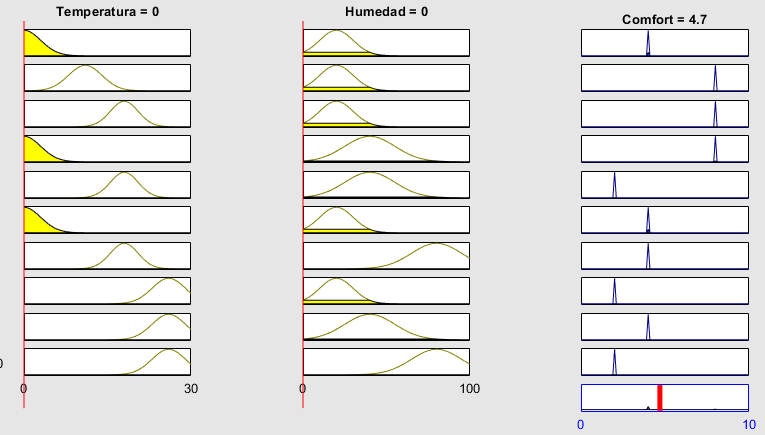
\includegraphics[width=1.4\textwidth]{IMG/RP21.png}
		\label{fig:G12}
	\end{subfigure}
	\hfill
	\begin{subfigure}{0.42\textwidth} % Reducido de 0.45
		\centering
		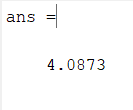
\includegraphics[width=0.8\textwidth]{IMG/M21.png}
		\label{fig:G13}
	\end{subfigure}
	\label{fig:comparacion6}
\end{figure}

A la izquierda se muestran los resultados del toolbox y a la derecha el resultado del sistema programado paso a paso. El toolbox reporta un valor de 4.7 para el caso planteado, mientras que el sistema programado paso a paso muestra un valor de 4.087. La diferencia entre ambos casos es de menos de 0.7 (menos de una unidad), por lo que se puede afirmar que llegan al mismo resultado. Una temperatura de 0 y una humedad de 0 llegan a dar como resultado un confort térmico de de 4.4 en promedio (Incomoda).

\newpage

\subsubsection{Caso medio}
Para el caso mínimo, se propone una $TEMPERATURA=15$ y una $HUMEDAD=50$ para ver como se comportan ambas versiones ante situación media.

\begin{figure}[h]
	\centering
	\begin{subfigure}{0.40\textwidth} % Reducido de 0.45
		\centering
		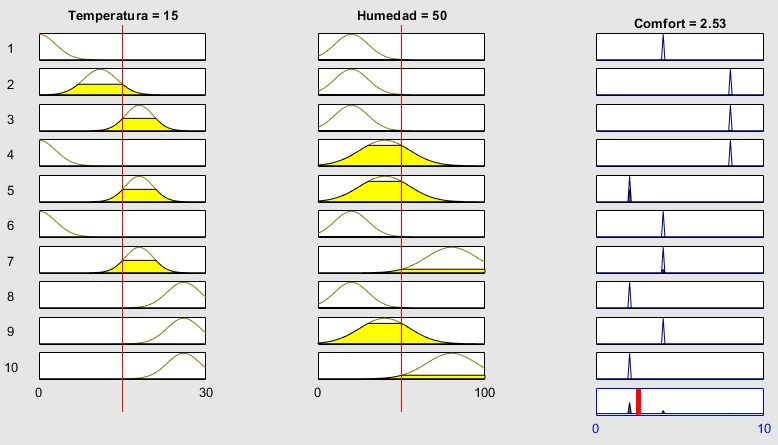
\includegraphics[width=1.4\textwidth]{IMG/RP22.png}
		\label{fig:G14}
	\end{subfigure}
	\hfill
	\begin{subfigure}{0.42\textwidth} % Reducido de 0.45
		\centering
		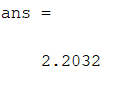
\includegraphics[width=0.8\textwidth]{IMG/M22.png}
		\label{fig:G15}
	\end{subfigure}
	\label{fig:comparacion7}
\end{figure}

A la izquierda se muestran los resultados del toolbox y a la derecha el resultado del sistema programado paso a paso. El toolbox reporta un valor de 2.53 para el caso planteado, mientras que el sistema programado paso a paso muestra un valor de 2.2032. La diferencia entre ambos casos es de menos de 0.3 (menos de una unidad), por lo que se puede afirmar que llegan al mismo resultado. Una temperatura de 15 y una humedad de 50 llegan a dar como resultado un confort térmico de de 2.35 en promedio (Malo).


\newpage

\subsubsection{Caso máximo}

Para el caso mínimo, se propone una $TEMPERATURA =  30$ y una $HUMEDAD = 100$ para ver como se comportan ambas versiones ante situaciones tan extremas.

\begin{figure}[h]
	\centering
	\begin{subfigure}{0.40\textwidth} % Reducido de 0.45
		\centering
		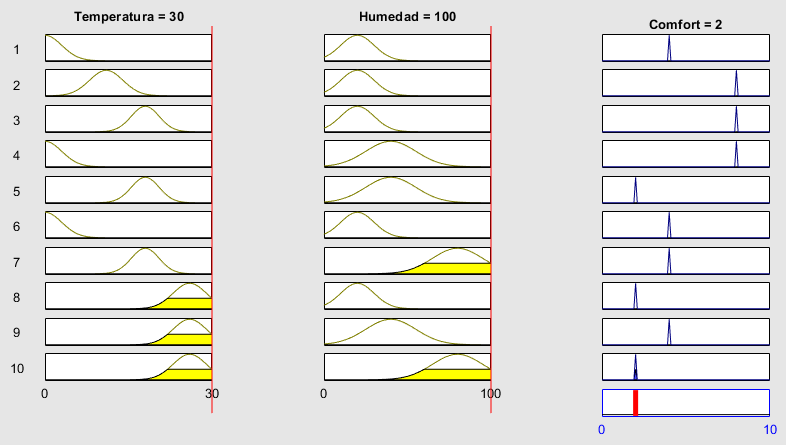
\includegraphics[width=1.4\textwidth]{IMG/RP23.png}
		\label{fig:G16}
	\end{subfigure}
	\hfill
	\begin{subfigure}{0.42\textwidth} % Reducido de 0.45
		\centering
		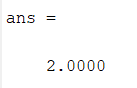
\includegraphics[width=0.8\textwidth]{IMG/M23.png}
		\label{fig:G17}
	\end{subfigure}
	\label{fig:comparacion8}
\end{figure}

A la izquierda se muestran los resultados del toolbox y a la derecha el resultado del sistema programado paso a paso. El toolbox reporta un valor de 2 para el caso planteado, mientras que el sistema programado paso a paso muestra un valor de 2. La diferencia entre ambos casos es nula, por lo que se puede afirmar que llegan al mismo resultado. Una temperatura de 30 y una humedad de 100 llegan a dar como resultado un confort térmico de de 2 (Malo).

\newpage


\section{Conclusiones}

A rasgos generales, los resultados del sistema programado y del toolbox de matlab resultan muy similares y no se alejan en más de una unidad.
Ambas propuestas son buenas, se tiene la sospecha que para el caso particular de la función de membresía Gaussiana puede que se este manejando alguna variante distinta entre el toolbox y el implementado, pero aun así llegan a resultados muy similares.

Por otro lado, la implementación del sistema supuso un reto en principio para asimilar toda la estructura que compone al sistema, el paso más complicado durante la realización de este trabajo fue el entender como deffuzificar la salida con el centro de masa. Una vez comprendido este punto, todo lo demás se traduce en la paciente y cuidadosa redacción de las funciones de membresía, la incorporación de sus parámetros y de la creación de las reglas.


\newpage

\section{Referencias}

\bibliographystyle{apalike}  % Estilo de cita, puedes cambiarlo si lo prefieres.
\bibliography{Biblio}         % Aquí incluyes el archivo .bib (sin extensión).

\newpage

\section{Anexos}

Este reporte se enviá con los códigos anexos que corresponden a:

\begin{enumerate}
	\item Archivo .fiz del sistema difuso para el problema 1 
	\item Código en matlab para ejecutar el sistema difuso programado para el problema 1
	\item Archivo .fiz del sistema difuso para el problema 2
	\item Código en matlab para ejecutar el sistema difuso programado para el problema 2
\end{enumerate}



\end{document}

